%---------------------------------------------------------------------
%
% Chapter 4: New techniques for multiobjective and goal-based search
%
%---------------------------------------------------------------------
%
% ChapContributions.tex
% Copyright 2015 Dr. Francisco J. Pulido
%
% This file belongs to the PhD titled "New Techniques and Algorithms for Multiobjective and Lexicographic Goal-Based Shortest Path Problems", distributed under the Creative Commons Licence Attribution-NonCommercial-NoDerivs 3.0, available in http://creativecommons.org/licenses/by-nc-nd/3.0/. The complete PhD dissertation is freely accessible from http://www.lcc.uma.es/~francis/
%
% This thesis has been written adapting the TeXiS template, a LaTeX template for writting thesis and other documents. The complete TeXiS package can be obtained from http://gaia.fdi.ucm.es/projects/texis/. TeXis is distributed under the same conditions of the LaTeX Project Public License (http://www.latex-project.org/lppl.txt). The complete license is available in http://creativecommons.org/licenses/by-sa/3.0/legalcode
%
%---------------------------------------------------------------------

\chapter{New techniques for multiobjective and goal-based search}
\label{chapContributions}


\begin{FraseCelebre}
\begin{Frase}
An algorithm must be seen to be believed.
\end{Frase}
\begin{Fuente}
Donald Knuth (1938-)
\end{Fuente}
\end{FraseCelebre}

This chapter describes the algorithmic contributions of this thesis.
%have been pointed out throughout this section. 
These are broadly aimed at an efficient solution of goal-based search problems. 
In the first place, we introduce a new algorithm that specifically searches for lexicographic goal solutions in Section \ref{chapMultiObjAlg:subsec:lexgo}. The algorithm is called \lexgo. We start noting that the optimality principle does not hold in general for lexicographic goal based preferences, and develop a specific pruning criterion for them. In the second place, we introduce in Section \ref{chapMultiObjAlg:sec:Time-efficient-MSalg} a dimensionality reduction technique that speeds up the time performance of Label-setting multicriteria search algorithms. We review the application of this technique to \namoa \ and \lexgo, in Sections \ref{chapMultiObjAlg:subsec:namoate} and \ref{chapMultiObjAlg:subsec:lexgote}, respectively. These algorithmic contributions are the base for the different alternatives to goal-based search analyzed later in this thesis.

%-------------------------------------------------------------------
\section{Algorithm \texorpdfstring{\lexgo}{LEXGO*}}
\label{chapMultiObjAlg:subsec:lexgo}
%-------------------------------------------------------------------

This section introduces \lexgo, an algorithm for lexicographic goal-based search problems. More precisely, we will address goal-based search according to the preferences already introduced in Section \ref{chapMultiObjAlg:subsec:lex-MOP}, and that will be used throughout this chapter. Multiobjective search algorithms benefit from the principle of optimality, i.e. an optimal path is made up of optimal subpaths. This property allows to drastically reduce the number of paths to be explored during search, pruning dominated alternatives at each node. Regrettably, the principle of optimality does not hold for lexicographic goal-based preferences. Let us see this by way of a simple example.

\begin{ejemplo}\label{ej:ejemplo-pruning1}
Let us consider a search problem in a multicriteria graph with start node $s$, a destination node $t$, and the following preferences over three different attributes:

   \begin{equation}
     \begin{array}{ccc}
       \textrm{Level 1:} & g_{1} \leq 20, & w_1 = 1.0 \\
       \textrm{Level 2:} & g_{2} \leq 20, & w_2 = 0.5 \\ 
                         & g_{3} \leq 20, & w_3 = 0.5 
     \end{array}
   \end{equation}

   Let us further assume the graph has two different paths $P_{1}$ and $P_{2}$ reaching some node $n$, where $\forall n \ \vec{h}(n) = (0, 0, 0)$, and the following costs and associated deviations:

   \begin{center}
   $\vec{g}(P_{1}) = \vec{f}(P_{1}) = (15, 16, 22) \ \Rightarrow
     \ \vec{d}(P_{1}) = (0,1)$ \\ 
   $\vec{g}(P_{2}) = \vec{f}(P_{2}) = (20, 12, 16) \ \Rightarrow
     \ \vec{d}(P_{2}) = (0,0)$ \\ 
   \end{center}

   We observe that $\vec{f}(P_{2}) \prec_{G} \vec{f}(P_{1})$, since $\vec{d}(P_{2}) \prec_{L} \vec{d}(P_{1})$. However, we cannot discard $P_1$ in favor of $P_2$. Let us now consider there is only one additional path $P_{3} = (n, \ldots, t)$ from $n$ to the destination node with cost $\vec g(P_3) = (4, 4, 4)$. It is easy to show now that the concatenation $P_1P_3$ is the only goal-optimal solution:

   \begin{center}
   $\vec{g}(P_{1}P_3) = (19, 20, 26) \ \Rightarrow
     \ \vec{d}(P_{1}P_3) = (0,3)$ \\ 
   $\vec{g}(P_{2}P_3) = (24, 16, 20) \ \Rightarrow
     \ \vec{d}(P_{2}P_3) = (4,0)$ \\ 
   \end{center}
\end{ejemplo} 

This is the main difficulty in the development of a specific goal-based search algorithm. According to our definition of goal-based preferences, goal optima are among Pareto optima. Therefore, pruning dominated paths will lead to a correct algorithm, although the number of explored paths is likely to be very similar to that of full Pareto search. Our aim is to introduce a specific pruning condition that allows us to reduce the number of paths explored in goal-based search and, more specifically, that guarantees that the set of paths explored in such search is a subset of the set of paths explored by a full Pareto search. 
Let us start introducing the fundamentals of this pruning preference. 

\begin{figure}[H]
%\centering
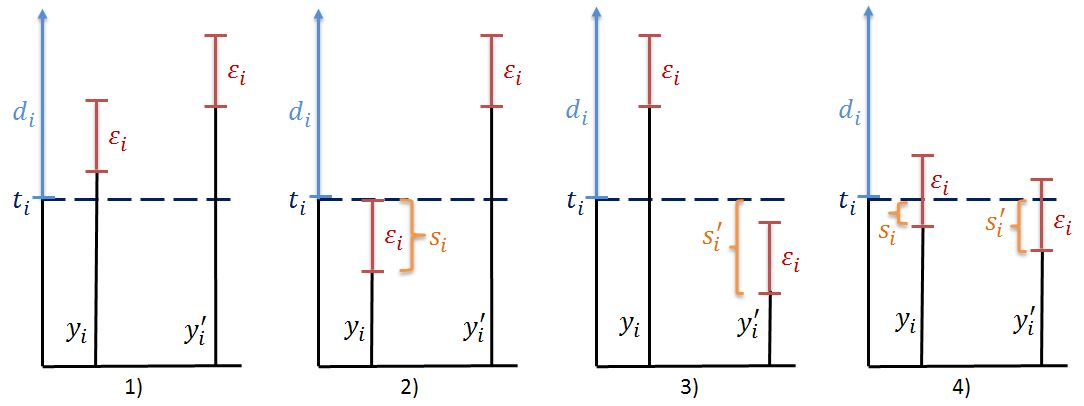
\includegraphics[width=1\textwidth]{Images/Chapter4/slack-variables}
\caption{ a) Graphic representation of slack variables for several scenarios where (1) $y_i, y'_i \geq t_i$, (2) $y_i \leq t_i < y'_i$, (3) $y'_i \leq t_i < y_i$ and (4) $y_i, y'_i < t_i$, adding $\epsilon_i$ to both $y_i$ and $y'_i$.}
\label{fig:2-2}
\end{figure}

\begin{defi}\label{chapMultiObjAlg:slacks}
Let us consider a goal $y_k \leq t_k$ over some measurable attribute $y_k$. The \textbf{slack variable} $s_k$ for this goal is defined as
\begin{equation}\label{eq:slack-def}
s_k = \max(0, t_k - y_k)
\end{equation}
Let us assume two vectors $\vec{y}, \vec{y'} \in \mathbb{R}^q$ and a level $j$ such that $d_j(\vec{y}) < d_j(\vec{y'})$. Let us denote 
$\Delta_j(\vec y, \vec{\epsilon}) = d_j(\vec{y} + \vec{\epsilon}) - d_j(\vec{y})$. Obviously, if \ $\vec{\epsilon} \succeq \vec{0}$, $\Delta_j(\vec y, \vec{\epsilon}) \geq 0$. We define the \textbf{cross-slack}  
$\delta_j(\vec{y},\vec{y'}) = \max_{\vec{\epsilon}\in \mathbb{R}^{+q}} (\Delta_j(\vec{y},\vec{\epsilon}) - \Delta_j(\vec{y'},\vec{\epsilon}))$, i.e. 
the greatest relative increment of the deviations of $\vec y$ and $\vec{y'}$ at level $j$ when adding any $\vec{\epsilon}\in \mathbb{R}^{+q}$. 
Notice that $\delta_j(\vec{y}, \vec{y'}) \geq 0$ and generally $\delta_j(\vec{y}, \vec{y'}) \neq \delta_j(\vec{y'}, \vec{y})$.

Each priority level $j$ comprises a set $I_j$ of one or more attributes $i$. Figure \ref{fig:2-2} shows that for each $i \in I_j$ four different cases can arise: (1) $y'_i, y_i \geq t_i$; (2) $y'_i \geq t_i$ and $y_i < t_i$; (3) $y'_i < t_i$ and $y_i \geq t_i$; (4) $y'_i, y_i < t_i$. It is straightforward that the greatest relative increment in cases 1 and 2 is 0, since the slack variable $s'_i$ equals $0$, while in cases 3 and 4, the greatest relative increment is 
$w_i \times (s'_i - s_i) = w_i \times (t_i - y'_i - (t_i - y_i)) =
w_i \times (y_i - y'_i)$. Therefore, an operative way of calculating the {\em cross-slack} $\delta_j(\vec{y}, \vec{y'})$ of $\vec{y}, \vec{y'}$ at level $j$ is

\begin{equation}\label{eq:slack-var}
    \delta_j(\vec{y}, \vec{y'}) = \sum_{k\in I_j} w_k \times \max(0, s'_k - s_k)
\end{equation}
\end{defi}

\begin{defi}\label{chapMultiObjAlg:pruningpreference}
We define the \textbf{pruning preference} $\prec_{P}$ by imposing on the lexicographical goal preference additional conditions concerning cross-slacks: 
    \begin{multline}\label{eq:cond-prune-new}
      \vec{y} \prec_{P} \vec{y'} \ \ \Leftrightarrow \ \ \exists j
      \ (d_j(\vec{y}) < d_j(\vec{y'}) \quad \land  \quad \delta_j(\vec{y}, \vec
      {y'}) < d_j(\vec{y'}) - d_j(\vec{y})    \\ \land      \quad \forall i < j
      \ \ (d_i(\vec{y}) = d_i(\vec{y'}) \ \quad \land \quad \delta_i(\vec{y}, \vec{y'}) = 0))
    \end{multline}
i.e., $\vec{y} \prec_{P} \vec{y'}$ when (i) $\vec{y} \prec_{G} \vec{y'}$;
(ii) the cross-slacks of  $\vec{y}$ and  $\vec{y'}$ are zero for the first levels (where deviations are the same); and (iii) for the first level where deviations differ, the cross-slack of $\vec{y}$ and $\vec{y'}$ is strictly smaller than the difference between deviations. 

It can be easily checked that $\prec_{P}$ is irreflexive and  transitive. Therefore $\prec_{P}$ is a partial order relation. We read $\vec{y} \prec_{P} \vec{y'}$ as <<$\vec y$ allows to prune $\vec{y'}$>>.
\end{defi}

Table \ref{tab:pseudocode-lexgo} introduces \lexgo, an exact label-setting multicriteria search algorithm for lexicographic goal preferences with lower bound estimates. The inputs are a multiobjective graph $G$, a start node $s$, a destination node $t$, a set of weighted goals grouped in pre-emptive priority levels, and a monotone distance estimate function. \lexgo \ outputs the solution subgraph with the set of all goal-optimal solution paths between $s$ and $t$. In a similar manner than most of the multicriteria search algorithms presented in Section \ref{chapMultiObjAlg:sec:MSP}, the following data structures are managed by the algorithm:

\begin{itemize}
   \item \textbf{SG}: A search graph that records partial solution paths emanating from $s$ and their costs. Each node $n$ in $SG$ stores the following information:
	\begin{itemize}
   		\item $G_{op}(n)$: Set of cost vectors (labels) $\vec{g}_n$ of paths reaching node $n$ which have not been explored yet.
 		\item $G_{cl}(n)$: Set of labels reaching node $n$ which have already been explored.
	\end{itemize}

	\item \textbf{OPEN}: A priority queue of unexplored labels. For each node $n$ in $SG$ and each cost vector $\vec{g_n} \in G_{op}(n)$, there is a label $(n, \vec{g_n})$ in OPEN. In fact, labels are extended to include also evaluation vectors and their deviation from goals. Each extended label $(n, \vec{d}_n, \vec{f}_n, \vec{g}_n)$ denotes that node $n$ is reached by a path with cost $\vec{g}_n$, deviation vector $\vec{d}_n$, and evaluation vector $\vec{f}_n$. We define $\vec{f}_n = \vec{g}_n + \vec{h}(n)$.
For the sake of simplicity, we will denote $\vec{d}(\vec{f}_n)$ as $\vec{d}_n$. Initially, $(s, \vec{d}_s, \vec{f}_s, \vec{g}_s)$ is the only label in OPEN. Labels in OPEN are sorted lexicographically according to deviation vectors. In case of ties they are ordered lexicographically according to evaluation vectors $\vec f$. This ensures that the first element in the queue has a goal-optimal evaluation among all $f_n$ in OPEN.
	
	\item \textbf{COSTS}: The set of cost vectors of solution paths found to the destination node.
	
    \item \textbf{Best achievement} vector $\bestd$ \ among all solutions already found.
\end{itemize} 

The structure of \lexgo \ is similar to previous label-setting multicriteria algorithms with label expansion, but incorporating elements of lexicographic goal preferences to guarantee that only a subset of the labels explored by a full multicriteria search will need to be explored.

\begin{table}
\caption{Pseudocode of \lexgo \ algorithm }
\scalebox{.95}{
\begin{tabular}{p{\columnwidth}}
\hline
\begin{enumerate}
\item CREATE:
  \par ---An empty search graph $SG$, and set $s$ as its root.
  \par ---Two sets $G_{cl}(s) = \emptyset$ and $G_{op}(s)=
  \{\vec{0}\}$.   
  \par ---A list of alternatives, OPEN = $\{(s, \vec{d}(\vec{h}(s)), \vec{h}(s), \vec{0}\}$.
  \par ---An empty set, COSTS.
  \par ---$\bestd = \vec{\infty}$, optimum achievement vector for solutions found.

\item \label{lexgo:label-selection} PATH SELECTION. If OPEN is not empty, then, 

  \par ---Select a label $(n, \vec{d}_n, \vec{f}_n, \vec{g}_n)$ from
  OPEN such that \newline $\nexists (n', \vec d_{n'}, \vec{f}_{n'},
  \vec{g}_{n'}) \in OPEN$ such that $\vec{f}_{n'} \prec_{G} \vec{f}_n$.

  \par ---Delete the selected label from OPEN, and move $\vec g_n$ from $G_{op}(n)$ to $G_{cl}(n)$. 
  
  \par ---If \ $\exists \vec{c^*} \in COSTS$ such that $\vec{c^*} \prec
  \vec{f}_n$,  then repeat step \ref{label-selection}  (lazy filtering)
  

\item CHECK TERMINATION. If OPEN is empty, or
  $\bestd \prec_{L} \vec{d}_n$, then backtrack in $SG$ from $t$
  and return the set of solution paths with costs in COSTS.

\item SOLUTION RECORDING. If $n$ is a destination node, then
    \par ---Include $\vec g_n$ in COSTS.
    \par ---$\bestd \longleftarrow \vec{d}_n$
    \par ---Go back to step \ref{lexgo:label-selection}.

\item \label{path-expansion}PATH EXPANSION: If $n$ is not a destination node, then for all successor nodes $m$ of $n$ do:
    \begin{enumerate}
    \item Calculate the cost of the new path found to $m$, its
      evaluation vector and deviation, $\vec{g}_m = \vec{g}_n +
      \vec{c}(n,m)$,  $\vec{f}_m = \vec{g}_m + \vec{h}(m)$,
      $\vec{d}_m = \vec{d}(\vec{f}_m)$.

    \item If no Pareto or deviation filtering (equations \ref{eq:cond-filter-dom} and \ref{eq:cond-filter-new}), then:
      \begin{itemize}
      \item If $m \notin SG$: 
	\begin{itemize}
	\item Add $(m, \vec{d}_m, \vec{f}_m, \vec{g}_m)$ to OPEN
	\item Set $G_{op}(m)= \{(\vec{g}_m)\}$.
	\item Label with $\vec{g}_m$ a pointer from $m$ to $n$.
	\end{itemize}
      \item else if $\vec{g}_m$ equals some cost vector in  $G_{op}(m) \cup G_{cl}(m)$ then
	\begin{itemize}
	\item Label with $\vec{g}_m$ a pointer from $m$ to $n$.
	\end{itemize}
      \item else if no Pareto or deviation pruning (equations \ref{eq:cond-prune-dom} and \ref{eq:cond-prune-deviation}), then:  
	\begin{enumerate}
   \item Eliminate vectors \ $\vec{g'}_{m} \in G_{op}(m)$ such that $\vec{g}_m \prec \vec{g'}_{m} \ \lor \ \vec{f}_m \prec_P \vec{g'}_{m} + \vec{h}(m)$, and their corresponding labels $(m, \vec{d'}_{m}, \vec{f'}_{m}, \vec{g'}_{m})$ from OPEN.
	\item Add $(m, \vec{d}_m, \vec{f}_m, \vec{g}_m)$ to OPEN,
          $\vec{g}_m$ to $G_{op}(m)$ and label with $\vec{g}_m$ a
          pointer from $m$ to $n$.
	\end{enumerate}
      \end{itemize}
	\item Go back to step \ref{lexgo:label-selection}.
    \end{enumerate}        
\end{enumerate}
\\
\end{tabular}
}
\label{tab:pseudocode-lexgo} 
\end{table}

The algorithm has five main steps. The first one is devoted to data structure initialization. The second one is devoted to label selection from OPEN. At each iteration, the algorithm selects the first label  $(n, \vec{d}_n, \vec{f}_n, \vec{g}_n)$ from OPEN, which has a goal-optimal evaluation vector $f_n$. The label is removed from OPEN, and moved from $G_{op}(n)$ to $G_{cl}(n)$. The third step recovers and returns the solution subgraph whenever some termination condition is satisfied. The fourth step records the solution whenever a destination node is selected. COSTS and $\bestd$ are updated accordingly. Finally, the selected label is expanded in step \ref{path-expansion}, i.e. all the extensions of the selected label are considered for inclusion in the search graph and the OPEN set. 

The algorithm iterates over steps 2, 3 , 4 and 5 until OPEN is empty, or $\vec{d}_B \prec_{L} \vec{d}_n$, i.e. all potential goal-optimal solutions have been examined. In such case, the algorithm terminates returning a solution subgraph, made up of all goal-optimal solution paths. COSTS stores the set of distinct goal-optimal costs.
 
During path expansion two different conditions may prevent an extension from consideration: filtering and pruning. These are described in detail below. 

%-------------------------------------------------------------------
\subsection{Pruning conditions}
\label{subsubsec:Pruning-conditions}
%-------------------------------------------------------------------

As already explained in Example \ref{ej:ejemplo-pruning1}, the optimality principle does not hold for lexicographic goal preferences. Therefore, pruning and filtering using goal preferences would not yield an admissible label setting algorithm in this case. 
Nevertheless, \lexgo \ includes two pruning conditions that improve search efficiency and, at the same time, guarantee that no goal-optimal solution will be pruned, (see Theorem \ref{chapFormalAnalysis:teo:lexgo-admissible} in Section \ref{chapFormalAnalysis:sec:admissibilityLexgo}):

\begin{itemize}

  \item 
Pareto pruning. As in other Pareto search algorithms like \namoa, we prune any dominated path to any node. A new label $(m, \vec d_m, \vec f_m, \vec g_m)$ to node $m$ is pruned whenever

    \begin{equation}\label{eq:cond-prune-dom}
      \exists \vec g \in G_{op}(m) \cup G_{cl}(m) \ | \ \vec g \prec \vec g_m 
    \end{equation}
    
  \item 
Deviation-based pruning. We propose an additional specific pruning condition based in the pruning preference defined by equation \ref{eq:cond-prune-new}. We prune a new label $(m, \vec d_m, \vec f_m, \vec g_m)$ to node $m$ whenever

\begin{equation}\label{eq:cond-prune-deviation}
\exists \vec g \in G_{op}(m) \cup G_{cl}(m) \ | \ \vec g + \vec h(m)\prec_P \vec f_m   
\end{equation}
\end{itemize}


\begin{ejemplo}\label{ej:ejemplo-pruning2}
Let us assume the same preference as in Example \ref{ej:ejemplo-pruning1} and two paths $P$ and $P'$ reaching the same node $n$ from $s$ with the following evaluation vectors:

\begin{center}
$\vec f = \vec{f}(P) = (22, 22, 12) \Rightarrow \ \vec{d}(P) = (2,1)$ \\
$\vec f' = \vec{f}(P') = (22, 18, 26) \Rightarrow \ \vec{d}(P') = (2,3)$
\end{center}

We observe that $\vec{d}(P) \prec_L \vec{d}(P')$. We can also easily check that the extra conditions for pruning, $\delta_1(\vec{f}, \vec{f}') = 0$ and $\delta_2(\vec{f}, \vec{f}') = 1 < 3 - 1 = 2$, also hold,


\begin{displaymath}
  \begin{array}{ll}
    \delta_1(\vec{f}, \vec{f}') & = 1 \times \max(0, s_1' - s_1) = \max(0, 0-0)  = 0 \\
    \delta_2(\vec{f}, \vec{f}') & = 0.5 \times \max(0, s_2' - s_2) + 0.5 \times \max(0, s_3' - s_3) \\
                               & = 0.5 \times \max(0, 2-0) + 0.5 \times \max(0, 0-8) \\
                               & = 1 \\
  \end{array}
\end{displaymath}

Therefore, path $P'$ will never lead to a better solution than $P$ and can be safely pruned.
\end{ejemplo}

%-------------------------------------------------------------------
\subsection{Filtering conditions}
\label{subsubsec:Filtering-conditions}
%-------------------------------------------------------------------

Filtering is the process of discarding labels that will never lead to a solution better than one already found. Two different conditions allow a label $(n, \vec{d}_n, \vec{f}_n, \vec{g}_n)$ to be filtered:

\begin{itemize}
   \item Pareto filtering. This is the standard dominance filtering in Pareto search algorithms:
     \begin{equation}\label{eq:cond-filter-dom}
     \exists \vec{c^*} \in COSTS \ | \ \vec{c^*} \prec \vec{f}_n
     \end{equation}

   \item Deviation based filtering. We introduce a specific filtering condition for goal-based preferences when a known solution has better goal satisfaction:
     \begin{equation}\label{eq:cond-filter-new}
     \bestd \prec_{L} \vec{d}_n
     \end{equation}
\end{itemize}

When a new solution is found, or the best achievement vector is updated, no new label satisfying the above conditions will be allowed to enter OPEN, however, those labels already in OPEN will not be straightforwardly discarded. This is due to \lexgo \ applies \emph{lazy filtering}. 
%In broad terms, lazy filtering consists of avoiding looking through OPEN to discard those labels which are dominated by the solution found, instead, filter those labels when they are selected for expansion, since the former is more time consuming than the latter (using a priority queue to store labels in OPEN as reference).

%-------------------------------------------------------------------
\subsection{Example}
\label{chapMultiObjAlg:subsubsec:example}
%-------------------------------------------------------------------

Let us now illustrate the algorithm with a simple example. Let us assume that the decision maker's preference involves two levels of goals: \\
 
Level 1 \hspace{10 mm} $cost_{1}(P) \leq 10, \hspace{5 mm} w_{1} = 0.5$ \\
\hphantom{a} \hspace{26 mm} $cost_{2}(P) \leq 10, \hspace{5 mm} w_{2} = 0.5$ 

Level 2 \hspace{10 mm} $cost_{3}(P) \leq 10, \hspace{5 mm} w_{3} = 1$ \\

Let us consider the sample graph in Figure \ref{fig:2-3}, where $s$ is the start node, and $t$ the destination node. A lower bound function $\vec{h}(n)$ has been calculated using the method proposed by Tung and Chew \citep{Tung1992} and is presented in Table \ref{tab:h-example1}. A trace of the OPEN list is shown in Table \ref{tab:trace-example1}. At each iteration the selected label is indicated with an arrow and pruned labels are crossed out.

\begin{figure}[!ht]
\centering
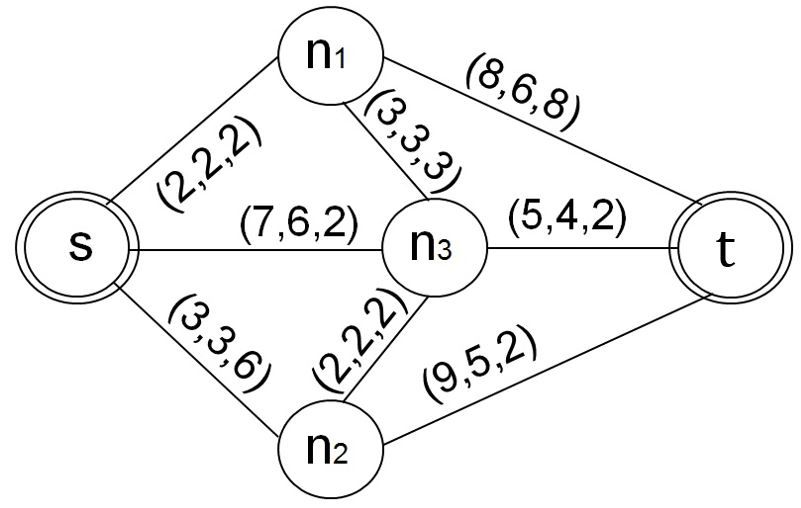
\includegraphics[width=0.5\textwidth]{Images/Chapter4/graph1}
\caption{Sample graph with satisfiable goals}
\label{fig:2-3}
\end{figure}

At iteration 1, SG has only node $s$ as its root and its corresponding label is selected from OPEN. Labels for the three descendants $n_1$, $n_2$ and $n_3$ of $s$ are added to OPEN. At iteration 2, two labels in OPEN have the same deviation vector, so the best lexicographic $\vec{f}$ is used to break the tie. Hence, the label to $n_1$ is selected. Its two successors $n_3$ and $t$ are added to OPEN. Addition of $n_3$ to $G_{op}(n_3)$ prunes the alternative already stored for $n_3$, since $(10,9,7) \prec_{P} (12,10,4)$. Notice that both evaluation vectors are non-dominated, however, the pruning condition presented in equation \ref{eq:cond-prune-deviation} is applied, since  $\delta_1((10,9,7),(12,10,4)) < d_1(12,10,4) - d_1(10,9,7) \ \Rightarrow \ 0 < 1-0$. At iteration 3, the label to $n_2$ is selected and expanded, generating new paths to the successors $n_3$ and $t$. The extension to $n_3$ is pruned, since the cost vector $(5,5,8)$ from path $(s, n_2, n_3)$ is dominated by the cost $(5,5,5)$ from path $(s, n_1, n_3)$. The second successor, $t$, is also pruned due to the existence of another label in $G_{op}(t)$ such that $(10,8,10) \prec_{P} (12,8,8)$. At iteration 4, the first path to a destination node is selected, the corresponding cost vector is added to COSTS $= \{ (10,8,10) \}$ and $\bestd$ is updated to $(0,0)$. This means that there is at least one path which satisfies all the goals provided. 

At iteration 5, $n_3$ is selected, and a new path to $t$ is generated and added to OPEN. At iteration 6, the only label in OPEN is selected. The cost vector $(10,9,7)$ represents another solution since $t$ is the destination node, its cost is not dominated by any vector in COSTS and it can also satisfy all goals. Finally, in the next iteration OPEN is empty and the algorithm would search backward from $t$ returning the solution subgraph with the two paths with costs (10,8,10) and (10,9,7).

\begin{table}
\caption{Lower bounds table with distance estimates of an example of \lexgo \ with satisfiable goals}
\centering
\begin{tabular}{cc}
\hline \noalign{\smallskip}
 n & $\vec h(n)$ \\
\noalign{\smallskip} \hline
$s$ & (10,8,4) \\
$n_1$ & (8,6,5)  \\
$n_2$ & (7,5,2)  \\
$n_3$ & (5,4,2)  \\
$t$ & (0,0,0)  \\
\hline
\end{tabular}
\label{tab:h-example1}
\end{table}

\begin{table}
\caption{Execution trace of an example of \lexgo \ with feasible goals (graph in Figure \ref{fig:2-3}).}
\centering
\begin{tabular}{ll}
\hline \noalign{\smallskip}
It & OPEN $(n,\vec{d},\vec{f},\vec{g})$ \\
\noalign{\smallskip} \hline
1 & $(s,(0,0),(10,8,4),(0,0,0))$ $\longleftarrow$ \\
\multirow{3}{*} {2} & $(n_1,(0,0),(10,8,7),(2,2,2))$ $\longleftarrow$\\
& $(n_2,(0,0),(10,8,8),(3,3,6))$ \\
& $(n_3,(1,0),(12,10,4),(7,6,2))$ \\
\multirow{4}{*} {3} & $(n_2,(0,0),(10,8,8),(3,3,6))$ $\longleftarrow$\\
& $(t,(0,0),(10,8,10),(10,8,10))$ \\
& $(n_3,(0,0),(10,9,7),(5,5,5))$ \\
& \sout{$(n_3,(1,0),(12,10,4),(7,6,2))$} \\
\multirow{4}{*} {4} & $(t,(0,0),(10,8,10),(10,8,10))$ $\longleftarrow$\\
& $(n_3,(0,0),(10,9,7),(5,5,5))$ \\
& \sout{$(n_3,(0,0),(10,9,10),(5,5,8))$} \\
& \sout{$(t,(1,0),(12,8,8),(12,8,8))$} \\
5 & $(n_3,(0,0),(10,9,7),(5,5,5))$ $\longleftarrow$\\
6 & $(t,(0,0),(10,9,7),(10,9,7))$ $\longleftarrow$ \\
7 & EMPTY SET\\
\hline
\end{tabular}
\label{tab:trace-example1}
\end{table}


%-------------------------------------------------------------------
\section{A dimensionality reduction technique for MSP}
\label{chapMultiObjAlg:sec:Time-efficient-MSalg}
%-------------------------------------------------------------------

This section describes a dimensionality reduction technique that speeds up the time performance of exact multicriteria search algorithms. Dimensionality reduction was first proposed as a space saving technique in the development of \emph{vector frontier search} \citep{Mandow2008,Mandow2009}, a blind multiobjective search algorithm that achieved impressive reductions in space requirements at the expense of increasing time requirements. This technique is used in this thesis showing that it can also be applied under reasonable assumptions to exact multicriteria search (and to \namoa \ and \lexgo \ in particular) to achieve important improvements in time performance. 

The key idea in dimensionality reduction is that, under a lexicographic order of expansion, dominance checks performed during filtering and certain pruning operations can be greatly simplified. We will start introducing the following useful terminology. We will say that  a vector $v$ is dominated by a set $X$ when there exists $v'\in X$ such that $v'\prec v$. Dominance checks performed on labels by \namoa (see Table \ref{ChapMultiObjAlg:tab:pseudocode-namoa}) can be stated as follows:
\begin{itemize}
    \item Filtering. Discard $(n,\vec g,\vec f)$ if $f$ is dominated by COSTS.
	 \item Op-pruning. Discard $(n,\vec g,\vec f)$ if $\vec g$ is dominated by $G_{op}(n)$.
	 \item Cl-pruning. Discard $(n,\vec g,\vec f)$ if $\vec g$ is dominated by $G_{cl}(n)$.
\end{itemize}

First we reproduce two definitions from \cite{Mandow2009}:

\begin{defi} \label{chapMultiObjAlg:def:tv}
Given a vector $ \vec v = (v_1, v_2, \ldots v_n)$, its \textbf{truncated vector} $ {t(\vec v)}$ is that vector $v$ without its first component, i.e. $ {t(\vec v)} = (v_2, \ldots v_n)$.
\end{defi}

\begin{defi} \label{chapMultiObjAlg:def:tv2}
Given a  set of vectors  $X$, its associated set of truncated vectors is  
$T(X) = \mathcal{N}(X)(\{ t(\vec x) | \; \vec x \in X\})$. 
\end{defi}

We call our reduction technique ``t-discarding'' (or \textit{truncated discarding}), since it is based on discarding cost vectors by their truncated cost vectors. 

\begin{defi}\label{chapMultiObjAlg:def:tv3}
Let $X$ be a set of vectors. A vector $\vec v$ is t-discarded by $X$ when for all $\vec{v'} \in X \ \ v'_1 \leq v_1$ and there is $\vec{v''}\in X$ such that $t(\vec{v''})\in T(X)$ and one of the following conditions holds:

a) $v''_1 < v_1$ and $t(\vec{v''}) \preceq t(\vec v)$; or

b) $v''_1 = v_1$ and $t(\vec{v''}) \prec t(\vec v)$.
\end{defi} 

\begin{ejemplo}
{\em
Figure \ref{fig:4-1} displays three cost vectors $ \vec x = (6, 2, 4)$, $ \vec y = (4, 4, 5)$, and $ \vec z = (2, 3, 6)$, and shows also their truncated vectors $ {t(\vec x)}$, $ {t(\vec y)}$, and $ {t(\vec z)}$. Notice that none of $\vec x, \vec y, \vec z$ dominates any of the others;
so $\mathcal{N}(X)=\{\vec x,\vec y,\vec z\}$. On the other hand the truncated vectors are $t(\vec x)=(2,4)$, $t(\vec y)=(4,5)$ and $t(\vec z)=(3,6)$. Since ${t(\vec y)}$ and ${t(\vec z)}$ are dominated by ${t(\vec x)}$ we have $T(X)= \{(2,4)\}$. 

Let us consider now  a vector $\vec w=(7,2,4)$. The standard dominance test would imply three vector comparisons in the worst case,
namely those of $\vec w$ against $\vec x, \vec y$ and $\vec z$. However, t-discarding implies just one vector comparison, that of $t(\vec w)$ against $t(\vec x)$.
Since $t(\vec x) \preceq t(\vec w)$ and $x_1 < w_1$, $w$ will be t-discarded by $X$.

Let us consider now vector $w'=(6,2,4)$. Let us check if $\vec{w'}$ is t-discarded by $X$. We have $t(\vec x) \preceq t(\vec{w'})$, but $x_1 \not< w'_1$, so condition (a) does not hold. Again, $t(\vec x) \not\prec t(\vec{w'})$, so condition (b) does not hold either, and in consequence $\vec{w'}$ is not t-discarded by $X$.
}
\end{ejemplo}

\begin{figure}%[ht]
\centering
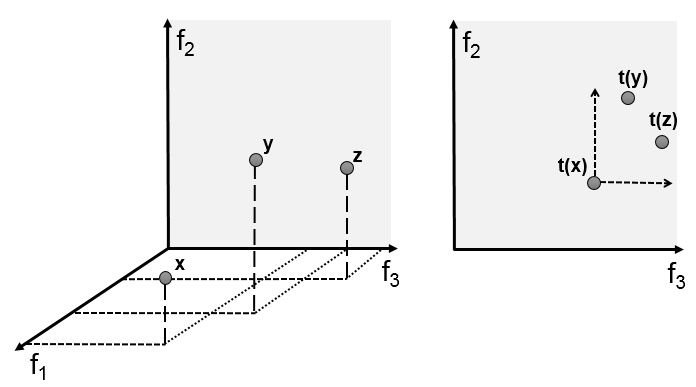
\includegraphics[width=0.75\textwidth]{Images/Chapter4/vectors}
\caption{A set of vectors $X = \{\vec x,\vec y,\vec z\}$ and its truncated vectors $t(\vec x),t(\vec y),t(\vec z)$.}
\label{fig:4-1}
\end{figure}

We propose a modification of filtering and/or cl-pruning checks and prove that the new version of the checks is equivalent to the original one, given some assumptions, see the formal proof in Section \ref{chapFormalAnalysis:sec:admissibilityNamoate}. An example concerning the impossibility of applying t-discarding to the op-pruning is shown in Section \ref{chapMultiObjAlg:subsec:namoate}, while the relative ratio of op-pruning, cl-pruning and filtering operations over the total number of discarded labels in our experiments over random grids and road maps can be seen in Figures \ref{fig:6-9} and \ref{fig:7-4}, respectively.

We present below the application of the t-discarding technique to \namoa. 
Moreover, let us emphasize that not only a priori multicriteria algorithms may benefit from this technique, we also review the application to \lexgo \ in Section \ref{chapMultiObjAlg:subsec:lexgote}.

%-------------------------------------------------------------------
\section{Algorithm \texorpdfstring{\namoate}{NAMOA*te}}
\label{chapMultiObjAlg:subsec:namoate}
%-------------------------------------------------------------------

Table \ref{ChapMultiObjAlg:tab:pseudocode-namoa-te} shows a slightly modified pseudocode of \namoa \ combined with the dimensionality reduction technique, i.e. \namoate. The newly added or modified pseudocode lines have been emphasized with a right arrow. Although \namoa \ uses a general lower bound function $H(n)$ that returns a set of vector estimates, \namoate \ employs a lower bound function $h(n)$, limited to a single vector estimate per node and that satisfies the monotone property (see Definition \ref{chapFormalAnalysis:def:multiObjmonotoneH}). \namoate \ uses the same data structures employed by \namoa, with the only addition of the sets T(COSTS) and $T(G_{cl}(n))$. 
%An example of \namoa \ run can be found in \citep[3.2]{Mandow2010} (the behaviour of \namoate \ is completely equivalent to \namoa).  

The new cl-pruning and filtering operations in \namoate \ employ the truncated set of vectors, instead of the original ones, to discard new labels. In addition, the truncated sets must be updated after each insertion of a new truncated vector. The equations corresponding to these operations are shown in Table \ref{ChapMultiObjAlg:tab:truncated-operations}. The update operation will be relatively costly depending on the size of the sets of truncated vectors. On the other hand, the size of the sets of truncated vectors over the size of the original ones defines the savings that can be achieved. This along with the frequency that op-pruning occurs shall define the efficiency of \namoate. We will analyze empirically the performance of \namoate \ in Sections \ref{chapEmpiricalAnalysis:sec:resultsgridsnamoate} and \ref{chapEmpiricalAnalysis:sec:resultsdimacsnamoate}. 

\begin{table}
\caption{New operations over truncated sets of vectors.}
\scalebox{.95}{
\begin{tabular}{p{\columnwidth}}
\hline
\begin{enumerate}
	\item Pareto pruning (dr). A label $(m,\vec f_m, \vec g_m)$ is pruned whenever     
		\begin{equation}\label{eq:trunc-cond-prune-dom-lexgo}
			\exists \vec v \in T(G_{cl}(m)) \ \ | \ \ v \prec t(\vec g_m) \qquad
			\lor \qquad \exists \vec g \in G_{op}(m) \ \ | \ \ \vec g \prec \vec g_m
		\end{equation}
	\item Pareto filtering (dr). A label $(m,\vec f_m, \vec g_m)$ is filtered whenever    
		\begin{equation}\label{eq:trunc-cond-filter-dom}
     		\exists \vec v \in T(COSTS) \quad | \quad \vec v \prec t(\vec f_m)
		\end{equation}
	\item Update set of truncated solution cost vectors. After inserting vector $\vec v$ in T(COSTS) do    
		\begin{equation}\label{eq:update-trunc-costs}
	      \text{Remove} \ \ \vec{v'} \in T(COSTS) \quad | \quad \vec v \prec \vec{v'}
		\end{equation}
	\item Update set of truncated permanent vectors. After inserting vector $\vec v$ in $T(G_{cl}(m))$ do
		\begin{equation}\label{eq:update-trunc-gcl}
	      \text{Remove} \ \ \vec{v'} \in T(G_{cl}(m)) \quad | \quad \vec v \prec \vec{v'}
		\end{equation}		
\end{enumerate}
\\
\end{tabular}
}
\label{ChapMultiObjAlg:tab:truncated-operations} 
\end{table}

Two important changes in the adaptation of \namoa \ should be noted. First, the lexicographic order is the mandatory label selection policy in \namoate \ to select between all non-dominated alternatives in OPEN, whilst \namoa \ can work out with any policy that assures the selected label is non-dominated. Moreover, \namoa \ has been previously reported to perform better under a linear aggregation policy than under a lexicographic one \citep{Machuca2011}. Second, in step \ref{ChapMultiObjAlg:pruning-namoa-te}, the original pseudocode of \namoa \ does not establish which pruning operation should be performed in the first place, over open or permanent labels, however, we plainly define the cl-pruning as the first operation to be made, to take advantage of the t-discarding technique before applying op-pruning. Concerning to op-pruning, let us now present an example to show why the new technique cannot be applied to the op-pruning operation.

\begin{table}
\caption{Pseudocode of $\text{NAMOA}_{dr}^*$ algorithm.}
\scalebox{.95}{
\begin{tabular}{p{\columnwidth}}
\hline
\begin{enumerate}
\item CREATE:
  \par --- An empty search graph SG, and place $s$ as its root.
  \par --- Two sets $G_{cl}(s) = \emptyset$ and $G_{op}(s)= \{(\vec{0})\}$.   
  \par --- A list of alternatives, OPEN = $\{(s, \vec{0}, \vec h(s)\} $.
  \par --- An empty set, COSTS.
  \par $\rightarrow$ Two empty sets of truncated vectors $T(G_{cl}(s))$ and T(COSTS).

\item \label{label-selection-namoa-te} PATH SELECTION. If OPEN is not empty, then, 

  \par $\rightarrow$ Select a label $(n, \vec g_n, \vec f_n) $ from OPEN such that $\nexists (n', \vec g_{n'}, \vec f_{n'}) \in$ OPEN such that $\vec f_{n'} \prec_L \vec f_n$.

  \par --- Delete the selected label from OPEN, and move $\vec g_n$ from $G_{op}(n)$ to $G_{cl}(n)$. 
  
  \par $\rightarrow$ Add $t(\vec g_n)$ to $T(G_{cl}(n))$ and update $T(G_{cl}(n))$ (equation \ref{eq:update-trunc-gcl}). 
  
  \par $\rightarrow$ If Pareto filtering (dr) $\vec f_n$ (equation \ref{eq:trunc-cond-filter-dom}), then repeat step \ref{label-selection-namoa-te}
  
\item CHECK TERMINATION. If OPEN is empty, then backtrack in SG from $\gamma$ and return the set of solution paths with costs in COSTS.

\item SOLUTION RECORDING. If $n$ is a destination node, then
    \par Include $\vec g_n$ in COSTS and 
    \par $\rightarrow$ Add $t(\vec g_n)$ to T(COSTS) and update T(COSTS) (equation \ref{eq:update-trunc-costs}). 
    \par --- Go back to step \ref{label-selection-namoa-te}.

\item PATH EXPANSION: If $n$ is not a destination node, then for all successor nodes $m$ of $n$ do:
  \begin{enumerate}
    \item Calculate the cost of the new path found to $m$ and its lower bound, \newline 
    $\vec g_m = \vec g_n + \vec c(n,m)$ and $\vec f_m = \vec g(m) + \vec h(m)$.
    \item $\rightarrow$ Unless Pareto filtering (dr) $\vec f_m$ (equation \ref{eq:trunc-cond-filter-dom}):
      \begin{enumerate}
      \item If $m \notin$ SG: 
	\begin{itemize}
	\item Set $G_{op}(m)= \{(\vec g_m)\}$ and add $(m, \vec g_m, \vec f_m)$ to OPEN.
	\item Label with $\vec g_m$ a pointer from $n$ to $m$.
	\end{itemize}
      \item else if $\vec g_m$ equals some cost vector in  $G_{op}(m) \cup G_{cl}(m)$ then
	\begin{itemize}
	\item Label with $\vec g_m$ a pointer from $n$ to $m$.
	\end{itemize}
      \item \label{ChapMultiObjAlg:pruning-namoa-te} $\rightarrow$ else unless Pareto pruning (dr) (eq \ref{eq:update-trunc-costs}):  
	\begin{itemize}
   \item Eliminate vectors $\vec g_{m'} \in G_{op}(m)$ such that $g_m \prec \vec g_{m'}$ and its corresponding label $(m, \vec g_{m'}, \vec f_{m'})$ from OPEN.
	\item Add $(m, \vec g_m, \vec f_m)$ to OPEN, $\vec g_m$ to $G_{op}(m)$ and label with $\vec g_m$ a pointer from $n$ to $m$.
	\end{itemize}
      \end{enumerate}
    \item Go back to step \ref{label-selection-namoa-te}.
  \end{enumerate}
\end{enumerate}
\\
\end{tabular}
}
\label{ChapMultiObjAlg:tab:pseudocode-namoa-te} 
\end{table}

\begin{ejemplo}\label{chapMultiObjAlg:ej:op-pruning}
Figure \ref{fig:2-4} displays a sample graph with three objectives. Let us assume for the sake of clarity that $\vec h(n) = \vec 0$. At iteration 1, $s$ is expanded and its two extended paths $s \rightarrow n_1$ and $s \rightarrow n_2$ stored in OPEN. At iteration 2, label $(n_1, (1,1,1), (1,1,1))$ is expanded and label $(n_3, (4,4,4), (4,4,4))$ recorded in $G_{op}(n_3)$. In case t-discarding were applied to op-pruning, $T(G_{op}(n_3)) = \{ (4,4) \}$. At the next iteration label $(n_2,$ $(2,2,2), (2,2,2))$ is expanded according to the lexicographic selection order. 

The new generated path, $s \rightarrow n_2 \rightarrow n_3$, with label $(n_3, (3,5,5), (3,5,5))$ is non-dominated with respect to $(n_3, (4,4,4), (4,4,4))$, however, if we apply op-pruning the truncated vector $(5,5)$ corresponding to label $(n_3, (3,5,5), (3,5,5))$ would be t-discarded by truncated vector $(4,4)$ corresponding to label $(n_3, (4,4,4), (4,4,4))$. Logically, the first component of the new generated label does not necessarily have its first component equal or greater than all the open labels reaching the node (on the contrary, a lexicographic order and a consistent lower bound function can guarantee that for the permanent labels), therefore, t-discarding cannot be applied to op-pruning.
\end{ejemplo}

\begin{figure}%[ht]
\centering
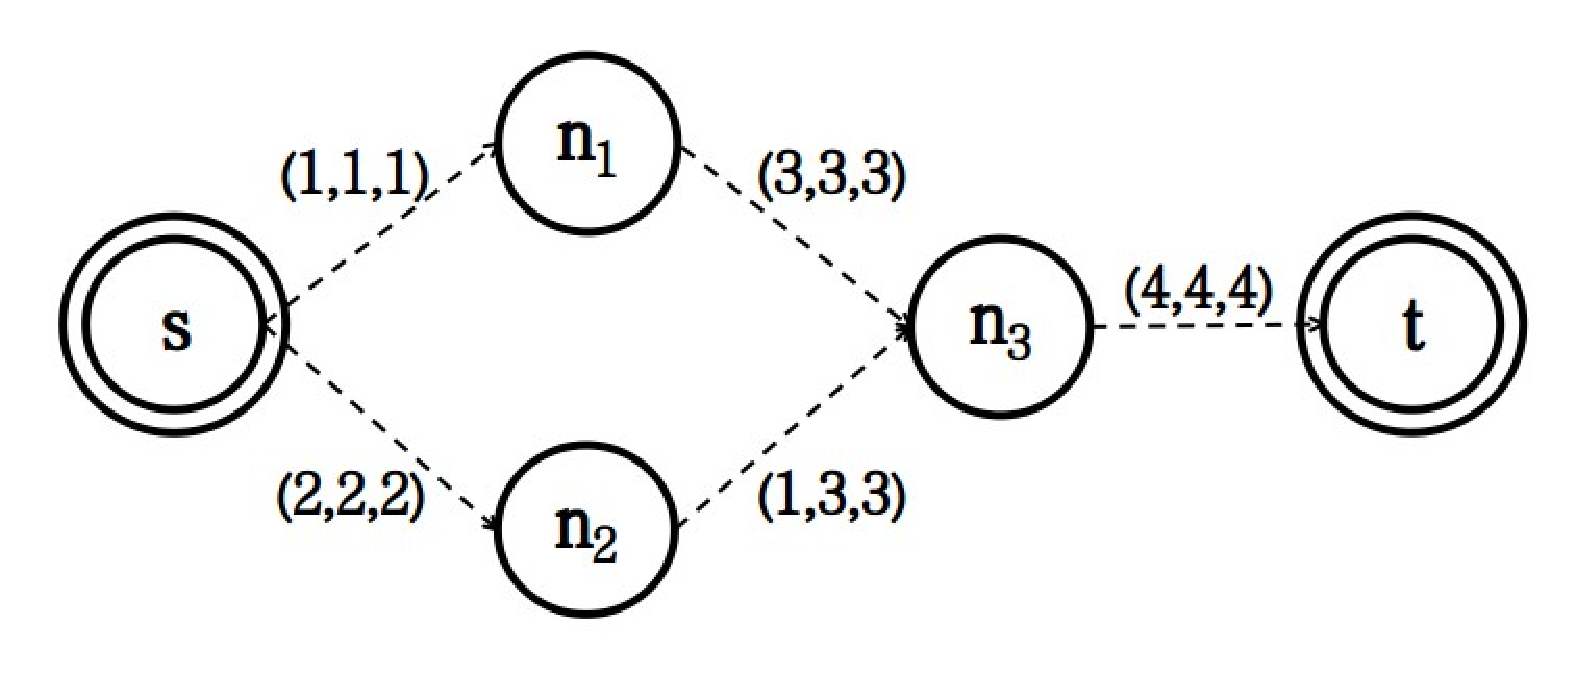
\includegraphics[width=0.65\textwidth]{Images/Chapter4/example-op-pruning}
\caption{Sample graph one with 3 objectives.}
\label{fig:2-4}
\end{figure}

%-------------------------------------------------------------------
\section{Algorithm \texorpdfstring{\lexgote}{LEXGO*te}}
\label{chapMultiObjAlg:subsec:lexgote}
%-------------------------------------------------------------------

Table \ref{tab:pseudocode-lexgo-te} displays the pseudocode of \lexgo \ adapted to incorporate the t-discarding procedure, i.e. the version that employs the dimensionality reduction technique, called \lexgote. A right arrow emphasizes the added or modified lines. The algorithm also uses the same monotone lower bound function $\vec h(n)$ and data structures employed by \lexgo, with the addition of T(COSTS) and $T(G_{cl}(n))$. An example of use of \lexgo \ was presented in Section \ref{chapMultiObjAlg:subsubsec:example} (the behavior of \lexgote \ does not differ from the behavior of \lexgo). 

\lexgo, like \namoa, can use any label selection policy as long as the selected labels are always guaranteed to be non-dominated. Nevertheless, \lexgote \ must employ the lexicographic order. This restricts the scenarios where cl-pruning and filtering operations can be applied to those where all permanent paths reaching a node have zero deviation for all priority levels, i.e. we define the scenario where t-discarding technique can be applied to \lexgote \ as follows:
\begin{equation}\label{eq:trunc-cond-prune-dom-lexgote}
	\forall n \ \ \forall l_n = (n, \vec d_n, \vec f_n, \vec g_n) \in (G_{cl}(n)) \quad \vec d_n = \vec 0 \quad \land \quad \forall \vec{c^*} \in COSTS \quad \vec{d}(\vec{c^*}) = \vec 0
\end{equation}
In this case, the set of labels expanded by \lexgo \ and \lexgote \ will be equivalent and they will be expanded exactly in the same order. Therefore, we will apply t-discarding to filtering or cl-pruning whenever all the labels in the set satisfy the condition to have a null deviation from goals. Since labels are expanded in lexicographic order, as soon as the first label with a positive  deviation is selected, \lexgote \ will change its filtering and cl-pruning to the regular one. We present an example of this phenomenon below. The analyses concerning the time performance of \lexgote \ over the other presented algorithms will be further studied empirically and formally in Section \ref{chapFormalAnalysis:sec:analysisLexgote}. 

\begin{table}
\caption{Pseudocode of \lexgote \ algorithm.}
\scalebox{.92}{  
\begin{tabular}{p{\columnwidth}}
\hline
\begin{enumerate}
\item CREATE:
  \par ---An empty search graph $SG$, and set $s$ as its root.
  \par ---Two empty sets $G_{cl}(s)$ and COSTS, and $G_{op}(s)=
  \{\vec{0}\}$.   
  \par ---A list of alternatives, OPEN = $\{(s, \vec{d}(\vec{h}(s)), \vec{h}(s), \vec{0}\}$.
  \par $\rightarrow$ Two empty sets of truncated vectors $T(G_{cl}(s))$ and T(COSTS).
  \par ---$\bestd = \vec{\infty}$, optimum achievement vector for solutions found.
  \par $\rightarrow$ A variable \textit{sat = TRUE} to record whether goals are satisfied or not. 

\item \label{lexgo-te:label-selection} PATH SELECTION. If OPEN is not empty, then, 

  \par Select a label $(n, \vec{d}_n, \vec{f}_n, \vec{g}_n)$ from
  OPEN s.t. \newline 
  $\nexists (n', \vec d_{n'}, \vec{f}_{n'}, \vec{g}_{n'}) \in OPEN$ \ | \ $\vec{f}_{n'} \prec_{G} \vec{f}_n$.

  \par ---Delete the selected label from OPEN, and move $\vec g_n$ from $G_{op}(n)$ to $G_{cl}(n)$. 
  
  \par $\rightarrow$ If $\vec d \neq \vec 0$ then \textit{sat = FALSE}.
  
  \par If \textit{sat == TRUE} then $t(\vec g_n)$ to $T(G_{cl}(n))$ and update $T(G_{cl}(n))$ (equation \ref{eq:update-trunc-gcl}). 
  	\begin{itemize}
  		\item If Pareto filtering (dr) $f_n$ (equation \ref{eq:trunc-cond-filter-dom}), then repeat step \ref{lexgo-te:label-selection}
  	\end{itemize}

  \par $\rightarrow$ Else if Pareto filtering (equation \ref{eq:cond-filter-dom}) then repeat step \ref{lexgo-te:label-selection}  
	  
\item CHECK TERMINATION. If OPEN is empty, or
  $\bestd \prec_{L} \vec{d}_n$, then backtrack in $SG$ from $t$
  and return the set of solution paths with costs in COSTS.

\item SOLUTION RECORDING. If $n$ is a destination node, then
    \par $\rightarrow$  Include $\vec g_n$ in COSTS and $\bestd \longleftarrow \vec{d}_n$
    \par $\rightarrow$ If \textit{sat} is TRUE add $t(\vec g_n)$ to T(COSTS) and update it (equation \ref{eq:update-trunc-costs}). 
    \par ---Go back to step \ref{lexgo-te:label-selection}.

\item PATH EXPANSION: If $n$ is not a destination node, then for all successor nodes $m$ of $n$ do:
    \begin{enumerate}
    \item Calculate the cost of the new path found to $m$, its evaluation vector and deviation, $\vec{g}_m = \vec{g}_n + \vec{c}(n,m)$,  $\vec{f}_m = \vec{g}_m + \vec{h}(m)$, $\vec{d}_m = \vec{d}(\vec{f}_m)$.
    \item If no Pareto or deviation filtering (equations \ref{eq:cond-filter-dom} (or \ref{eq:trunc-cond-filter-dom} when \textit{sat == TRUE}) and \ref{eq:cond-filter-new}), then:
      \begin{itemize}
      \item If $m \notin SG$: 
	\begin{itemize}
	\item Add $(m, \vec{d}_m, \vec{f}_m, \vec{g}_m)$ to OPEN
	\item Set $G_{op}(m)= \{(\vec{g}_m)\}$.
	\item Label with $\vec{g}_m$ a pointer from $m$ to $n$.
	\end{itemize}
      \item else if $\vec{g}_m$ equals some cost vector in  $G_{op}(m) \cup G_{cl}(m)$ then
	\begin{itemize}
	\item Label with $\vec{g}_m$ a pointer from $m$ to $n$.
	\end{itemize}
      \item else if no Pareto or deviation pruning (equations \ref{eq:cond-prune-dom} (or \ref{eq:trunc-cond-filter-dom} when \textit{sat == TRUE}) and \ref{eq:cond-prune-deviation}), then:  
	\begin{enumerate}
   \item Eliminate vectors \ $\vec{g'}_{m} \in G_{op}(m) \ \ |
          \ \ \vec{g}_m \prec \vec{g'}_{m} \ \lor \ \vec{f}_m \prec_P \vec{g'}_{m} + \vec{h}(m)$, and their corresponding labels $(m, \vec{d'}_{m}, \vec{f'}_{m}, \vec{g'}_{m})$ from OPEN.
	\item Add $(m, \vec{d}_m, \vec{f}_m, \vec{g}_m)$ to OPEN,
          $\vec{g}_m$ to $G_{op}(m)$ and label with $\vec{g}_m$ a
          pointer from $m$ to $n$.
	\end{enumerate}
      \end{itemize}
	\item Go back to step \ref{lexgo-te:label-selection}.
    \end{enumerate}        
\end{enumerate}
\\
\end{tabular}
}
\label{tab:pseudocode-lexgo-te} 
\end{table}

\begin{figure}%[ht]
\centering
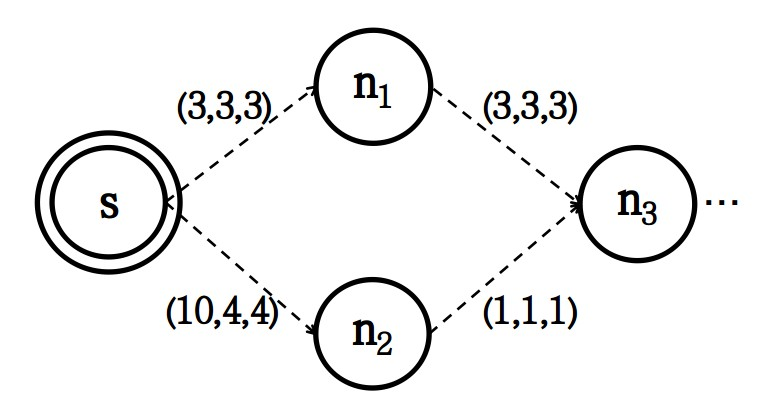
\includegraphics[width=0.5\textwidth]{Images/Chapter4/example-dev-op-pruning}
\caption{Sample graph two with 3 objectives.}
\label{fig:2-5}
\end{figure}

\begin{ejemplo}\label{chapMultiObjAlg:ej:dev-op-pruning}
Figure \ref{fig:2-5} displays a sample partial graph with three objectives. Let us assume that $\vec h(n) = \vec 0$ and the lexicographic goals are the ones presented in Section \ref{chapMultiObjAlg:subsubsec:example}. At iteration 1, $s$ is expanded and its two extended paths $s \rightarrow n_1$ and $s \rightarrow n_2$ stored in OPEN and labels ($n_1$, (0,0), (3,3,3), (3,3,3)) and ($n_2$, (0,0), (10,4,4), (10,4,4)), stored in $G_{op}(n_1)$ and $G_{op}(n_2)$, respectively.

At iteration 2, label ($n_1$, (0,0), (3,3,3), (3,3,3)) is expanded and label ($n_2$, (0,0), (6,6,6), (6,6,6)) recorded in $G_{op}(n_3)$. Thus,  At iteration 3, label ($n_3$, (0,0), (6,6,6), (6,6,6)) is expanded, since the concatenation of its deviation and evaluation vectors ($\vec d \cdot \vec f$) is lexicographically better than the other alternative in OPEN, ($n_2$, (0,0), (10,4,4), (10,4,4)), and added to $G_{cl}(n_3)$.

At iteration 4, label ($n_2$, (0,0), (10,4,4), (10,4,4)) is expanded and its extension ($n_2$, (0.5,0), (11,5,5), (11,5,5)) is checked for a cl-pruning operation against $G_{cl}(n_3) = \{((0,0), (6,6,6), (6,6,6)) \}$. If we do not pay attention to the fact that not all deviation vectors of labels in $n_3$ are zero, the condition to t-discard this path applies, i.e. $(5,5) \prec (6,6)$, but it is obvious that $(11,5,5) \nprec (6,6,6)$. 
\end{ejemplo}


